\documentclass{article}
\usepackage[utf8]{inputenc}
\usepackage{graphicx}
\usepackage{amsmath}
\usepackage{parskip}
\usepackage{tabularx}
\usepackage[most]{tcolorbox}
\usepackage{graphicx,wrapfig,lipsum}
\graphicspath{ {images/} }

\begin{document}
\begin{center}
\huge\bf Elliptic Curve Cryptography 
\newline
\newline
\end{center}




% Author --- SABVA JAY DILIPBHAI

\begin{center}
   
    \setlength{\fboxrule}{.5mm}\setlength{\fboxsep}{1.2mm}
	\newlength{\boxlength}\setlength{\boxlength}{\textwidth}
	\addtolength{\boxlength}{-4mm}
	\begin{center}\framebox{\parbox{\boxlength}{\bf
             	Professors: Manish Gupta\\[10pt]
				Group Members and their Contribution
				\newline
				\begin{enumerate}
				    \item Soham Viradiya(202101472)\\
				    Contribution:
				    \newline 
				    
				    \item Jay Sabva(202101224)\\
				    Contribution:
				    \newline
				    
				    \item Shrut Kalathiya(202101479)\\
				    Contribution:
				    \newline
				    
				    \item Vasu Golakiya(202101487)\\
				    Contribution:
				    \newline
				    \item Vandit Bhalani(202101478)\\
				    Contribution: 
				    \newline
				    \item Dev Changela(202101069)\\
				    Contribution:
				    \newline
				    \item Swet Lakhani(202101218)\\
				    Contribution:
				    \newline
				    
				\end{enumerate}
	}}
	\end{center} 
	\vspace{5mm}
\end{center}

% Author --- SABVA JAY DILIPBHAI




\newpage
\section{Introduction and History of Cryptography}
The two eras in the history of cryptography are the classical era and the modern era.The introduction of the RSA algorithm and the Diffie-Hellman key exchange algorithm in 1977 established the separation of the two.These new algorithms were earth-shattering because they were the first effective cryptographic algorithms whose security was based on the theory of numbers;they were also the first to make it possible for two parties to communicate securely without sharing a secret.When it comes to communication between any two parties,cryptography has advanced from being used to safely carry codebooks around the globe to allowing for provably secure key exchanges between two parties.

The basis of modern cryptography is the concept that the key used to encrypt data may be made public but the key required to decode it can be kept secret. These systems are referred to be public key cryptography systems as a result. The first and currently most popular of these systems is called RSA, after the names of the three individuals who initially revealed the algorithm to the public: Ron Rivest, Adi Shamir, and Leonard Adleman.
% Author --- SABVA JAY DILIPBHAI
A group of algorithms that are simple to process in one way but difficult to reverse is necessary for a public key cryptography system to function. The simple procedure for RSA multiplies two prime values. Factoring the product of the multiplication into its two component primes is the tough pair algorithm, if multiplication is the simple method. Trap door Functions are a set of algorithms that are fast in one direction and difficult in the other. Creating a safe public key cryptography system requires finding a decent trapdoor function.Simply said, a cryptographic system based on a Trapdoor Function will be more secure the greater the difference between the complexity of moving in one way and going in the other.
\begin{figure}[hb]
  \centering
  \begin{minipage}[hb]{0.3\textwidth}
    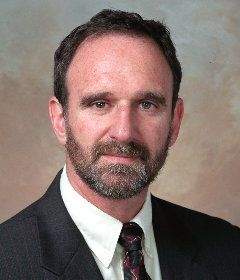
\includegraphics[width=\textwidth]{Martin-Hellman.jpg}
    \caption{Martin Hellman}
  \end{minipage}
  \hfill
  \begin{minipage}[hb]{0.3\textwidth}
    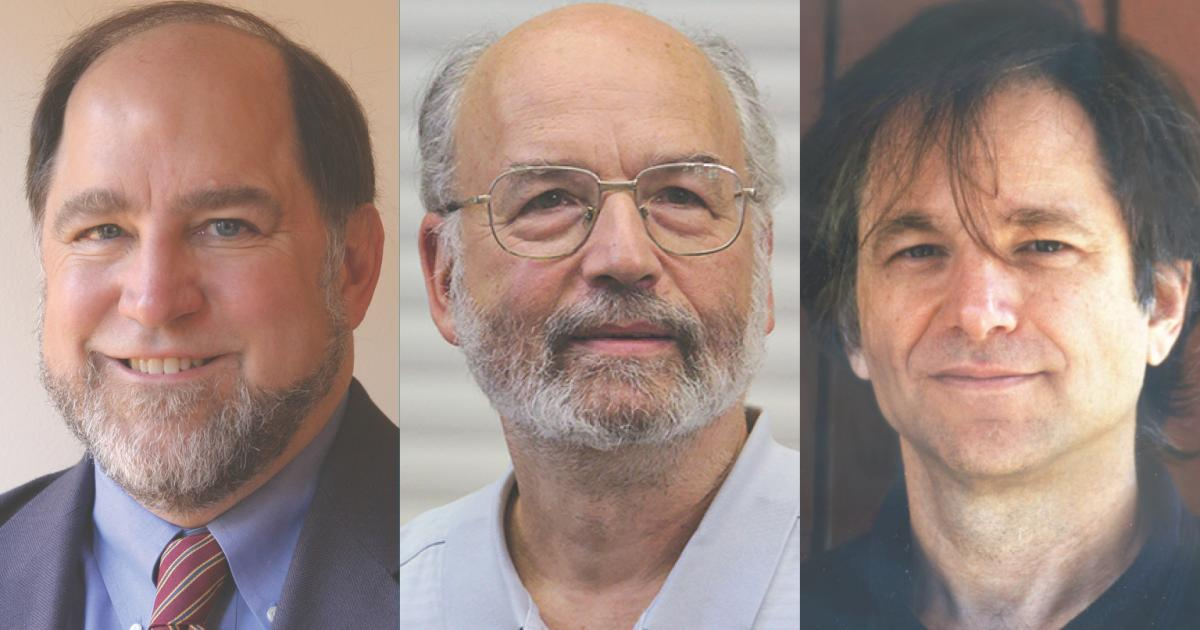
\includegraphics[width=\textwidth]{RSA.jpg}
    \caption{Rivet-Shamir-Adleman}
  \end{minipage}
  \hfill
  \begin{minipage}[hb]{0.3\textwidth}
    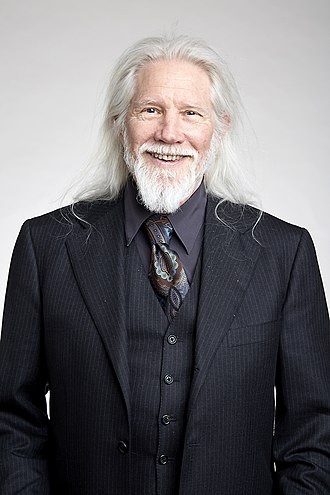
\includegraphics[width=\textwidth]{Diffle.jpg}
    \caption{Whitefield Diffle}
  \end{minipage}
\end{figure}

\section{RSA algorithm}
A widely used public-key cryptosystem for secure data transfer is RSA (Rivet-Shamir-Adleman). The names Ron Rivest, Adi Shamir, and Leonard Adleman, who first publicly revealed the algorithm in 1977, are the source of the abbreviation "RSA." The encryption key of a public-key cryptosystem is distinct from the decryption key, which is kept confidential (Private). A user of RSA generates and distributes a public key based on two significant prime numbers and an auxiliary value. It is a hidden what the prime numbers are. Anyone can encrypt messages using the public key, but only someone who is familiar with the prime numbers can decode them.
The "factoring issue," which is the practical challenge of factoring the product of two huge prime numbers, is the foundation for RSA security.
The RSA problem is the process of deciphering RSA encryption.. It is arguable if it is pretty hard as the factoring problem. If a sufficiently enough key is shared, the system cannot be attacked using any known techniques. The RSA algorithm operates quite slowly.

Let's use an illustration to help make this more clear. If we combine the prime numbers 13 and 7, we get our maximum value of 91. Let's say that the number 5 is our public encryption key. The Extended Euclidean Algorithm is then used to determine that the private key is the number 29, given the knowledge that 7 and 13 are factors of 91.
% Author --- SABVA JAY DILIPBHAI

\hspace{1cm}
\begin{centre}
\boxed{public \:key\:(e)\,:5\quad private\:key\;(d)\,:29\quad maximum\:key\:(n)\,:91}
\end{centre}

Let's use these values to encrypt the message "$CLOUD$" by encrypting the values.
We must convert the characters into numbers in order to represent a message numerically.UTF-8 is a popular way to represent the Latin alphabet.A number is assigned to each character.
\begin{figure}[h]
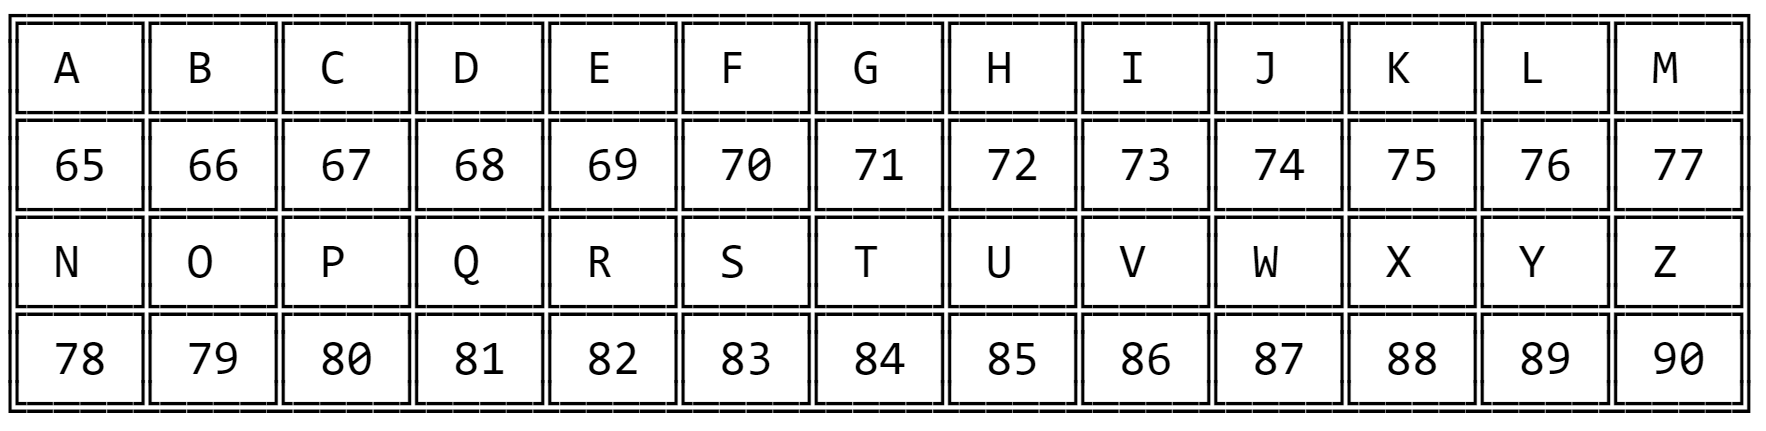
\includegraphics[width=10cm, height=2.5cm]{ASCII.png}
\centering
\end{figure}

$CLOUD$ is 67,76,79,85,68 in this encoding. These numbers may all be encrypted separately because they are all less than our limit of 91. Let's Start with the initial letter,
To obtain the encrypted value for $C$=67, we must multiply it by itself five times (using the public key).

\begin{centre}
\boxed{\(Encrypted\:Data\:E\, = A^e*(mod n)\)}
\hspace{0.8cm}
\boxed{\(Decrypted\:Data\:D\,= L^d*(mod n)\)}
\end{centre}


\(Encrypted\:Data\:C\,=67^5mod91=58\) \hspace{0.6cm} \(Decrypted\:Data \:C\,=58^{29}mod91=67\)\\
\(Encrypted\: Data\: L\,=76^5mod91=20\) \hspace{0.6cm} \(Decrypted\:Data \:L\,=20^{29}mod91=76\)\\
\(Encrypted\: Data \:O\,=79^5mod91=53\) \hspace{0.6cm} \(Decrypted\:Data \:O\,=53^{29}mod91=79\)\\
\(Encrypted\: Data\: U\,=85^5mod91=50\) \hspace{0.6cm}\(Decrypted\:Data \:U\,=50^{29}mod91=85\)\\
\(Encrypted \:Data\: D\,=68^5mod91=87\) \hspace{0.6cm} \(Decrypted\:Data \:D\,=87^{29}mod91=68\)\\

Therefore, it is clear that the keys are not symmetric, makes decryption more difficult.
\subsection{Encryption}
Let's say Alice wants to tell her buddy Bob something private.A single letter "C" is the message.
Assuming that her sworn enemy Eve may read this letter while it is in transit, how can she deliver it in confidence?
% Author --- SABVA JAY DILIPBHAI

$Example$:
The public key, or "Lock" (5,14)
Alice (the sender) uses this public pair of numbers to encrypt messages.
The private key is the "Key"
(17,14)
This pair's first number is private, meaning that only Bob is aware of it (the receiver).
To decrypt messages, this pair is used.
\begin{enumerate}
  \item The message "C" is encrypted by Alice using (5,14).

a. "C" is first converted into an integer."C" corresponds to the number 67 in ASCII.
To keep things simple, let's assume it maps to 3 instead.

b.3 is then encrypted \(3^5mod(14)=5\)
  \itemBob receives the result, 5, from Alice. Even if Eve peeks and notices this message, it says nothing to them.
  \item Bob uses the resulting decryption to (17,14).

a.\:\(5^{17}mod(14)=3\)

b.The result is 3.
To obtain the original message, Bob maps 3 back to a character, which is "C".
\end{enumerate}
\subsubsection{Lock & Key Generation}
Bob generates these two points of number in our illustration. So that only he can decrypt messages, he makes the first pair of numbers (5,14) publicly available to everyone while keeping the second pair of numbers (17,14) secret.
\begin{enumerate}
  \item Bob Pick $p$ and $q$, two prime numbers. They should be large in real-world scenarios (for security), but we'll pick modest numbers to make things simpler.
  \begin{center}
      \boxed{p=2\quad q=7}
  \end{center}
  \item Compute \begin{center}
      \boxed{n=p*q}
  \end{center} 
  \item Compute $e$(for encryption) such that:
  \begin{center}
      \boxed{1<e<(p-1)(q-1)\quad\quad and  \quad\quad GCD(e,(p-1)(q-1)=1}
  \end{center}
  \item Compute $d$ (for decryption) such that:
  \begin{center}
      \boxed{d=e^{-1}mod((p-1)(q-1))}
      \newline
      \newline
      \boxed{d*5=1mod6}
  \end{center}
  This means d can be 5,or 11,or 17,and so on.We"ll choose d=17.
  That's it,we're done
  \begin{center}
      \hspace{1.6cm}\boxed{The\: "Lock"\::(e,n)\,=\,(5,14)}
      \newline
      \newline
      \boxed{The\: "Key"\::(d,n)\,=\,(17,14)}
  \end{center}
As clearly explained, messages may be encrypted by senders using the first pair of numbers, and decrypted by receivers using the second set of numbers.
  
  The fundamental idea behind RSA is that it is possible to obtain positive numbers e, d, and n such that \((m^{e} \:mod\: n)^d \:mod \:n = \:m\) and such that even if e and n are made public, it would be very difficult to figure out what d is
\end{enumerate}
The key point is that you may take a number, multiply it by itself a certain number of times to get a totally arbitrary number, and then multiply that number by itself a different, secret number of times to return to the original number.
As the size of the numbers being factored increases, these algorithms become more effective.
As the number (the key's bit length) grows more, the difference in difficulty between multiplying large numbers and factoring large numbers is less.
The size of the keys must expand even more quickly as the resources available to decipher numbers grow.
For portable, low-power devices with limited processing capability, this is an unsustainable position.
Factoring and multiplication are separated by an impossible distance.
\subsection{Issues with RSA}
The largest number factored as of 2005 is 663 bits long and was done so using distributed methods that are state-of-the-art. Although argued, experts believe that 1024-bit keys may eventually become breakable. Using a home computer, 256-bit length keys may be cracked in a short amount of time. The 2048-bit key length is currently proposed [wik]. Although most personal computers are not affected by this length, it renders low processing power portable devices like smartcards ineffective. In these devices, there are limitations on processor word length, available memory, and clock speeds.It became necessary to develop a system that provided the same level of cryptographic security with shorter key lengths as the requirement for portable and secure identification progressively becomes a need and as RSA key sizes will increase in proportion to the processing power available. One such method is ECC, which is discussed in the section below.

All of this simply indicates that RSA is not the best solution for the cryptography of the future.

In a perfect trapdoor function, the difficulty of the easy and difficult paths increases according to the numbers under consideration.
\newpage
\section{Diffie-Hellman key exchange}
\subsection{Introduction}
In order to solve the issue of key agreement and exchange, Whitefield and Martin Hellman developed the Diffie-Hellman key exchange algorithms in 1976. After Whitefield Diffe and Martin Hellman, it was one of the earliest public-key exchange protocols developed by Ralph Merkle. It makes it possible for the two parties to agree on a symmetric key and communicate with one another (a key that can only be used for encrypting and decrypting).
% Author --- SABVA JAY DILIPBHAI
This algorithm cannot be used for encryption or decryption; it can only be used for key exchange. Mathematical concepts are the foundation of the algorithm.
\subsection{Reason to use Algorithm}
A key can be attacked between the instant it is being sent and received (i.e. Insecurity may occurs). It enables the establishment of a shared secret key across an unsecure channel by two people with no prior knowledge.
\subsection{General Overview of an algorithm}

\begin{wrapfigure}{r}{4.8cm}
\caption{Illustration of Diffie-Hellman key exchange}
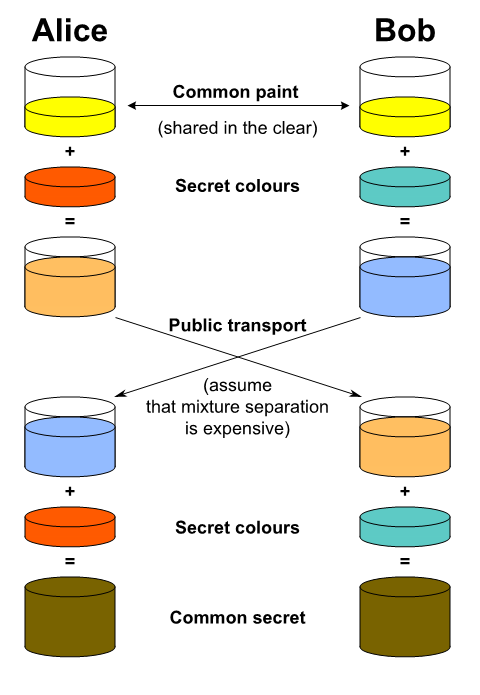
\includegraphics[width=5cm,height=7cm]{Color.png}
\end{wrapfigure} 
Publicly agreeing on a random starting colour that is not private, Alice and Bob (but should be different every time). Yellow is used as an example. Additionally, each participant chooses a secret colour that they keep to themselves; in this example, the colours are red and cyan. The key step in the procedure is when Alice and Bob mix their respective secret colours with the colour they both share to produce combinations of orange-tan and light blue, respectively, before publicly exchanging the two colours. Finally, they each combine their personal colour with the color they received from their buddy. The outcome is a final colour mixture (in this example, yellow-brown) that is the same as their partner's final colour mixture.
It would be challenging for a third party to determine the final secret colour from the exchange if it just knew the common colour (yellow) and the first mixed colours (orange-tan and light blue) (yellow-brown).
\subsection{Mathematical Explanation}
The multiplicative group of integers modulo $p$, where $p$ is prime, and $g$ is a primitive root modulo $p$ are used in the protocol's initial and most basic implementation. In assure that the resulting shared secret can have any value between 1 and $p-1$, these two values were selected in this manner. Here is an illustration of the protocol,with non-secret values: \textcolor{blue}{blue},and secret values in \textcolor{red}{red}
\begin{enumerate}
    \item Here Alice and Bob wants to share there secret but Eve is keeping watch on Them So Alice and Bob publicly agree to use a modulus \textcolor{blue}{$p$=23} and base \textcolor{blue}{$g=5$}(primitive root of modulo 23).
    \item Alice choose a secret integer \textcolor{red}{$a=4$},then sends Bob \textcolor{blue}{\(A=g^\textcolor{red}{a}\)}\:mod\,\textcolor{blue}{$p$}
    \begin{itemize}
        \item \textcolor{blue}{\(A=5^\textcolor{red}{4}\)}\:mod\,\textcolor{blue}{23=4}
\end{itemize}
    \item Bob choose a secret integer \textcolor{red}{$b=3$},then sends Alice \textcolor{blue}{\(B=g^\textcolor{red}{b}\)}\:mod\,\textcolor{blue}{$p$}
    \begin{itemize}
        \item \textcolor{blue}{\(B=5^\textcolor{red}{3}\)}\:mod\,\textcolor{blue}{23=10}
\end{itemize}
    \item Alice computes \textcolor{red}{$s$}\textcolor{blue}{\(=B^\textcolor{red}{a}\)}\:mod\,\textcolor{blue}{$p$}
    \begin{itemize}
        \item \textcolor{red}{$s$}\textcolor{blue}{\(=10^\textcolor{red}{4}\)}\:mod\,\textcolor{blue}{23}=\textcolor{red}{18}
    \end{itemize}
    \item Bob computes \textcolor{red}{$s$}\textcolor{blue}{\(=A^\textcolor{red}{b}\)}\:mod\,\textcolor{blue}{$p$}
    \begin{itemize}
        \item \textcolor{red}{$s$}\textcolor{blue}{\(=4^\textcolor{red}{3}\)}\:mod\,\textcolor{blue}{23}=\textcolor{red}{18}
    \end{itemize}
    \item Alice and Bob now share a secret
\end{enumerate}
Both Alice and Bob arrived at the same values because under mod $p$,
\begin{center}
    \boxed{\textcolor{blue}{\(A^\textcolor{red}{b}\)}\:mod\,\textcolor{blue}{$p$}\:\:\textcolor{blue}{\(=g^\textcolor{red}{ab}\)}\:mod\,\textcolor{blue}{$p$}\:\textcolor{blue}{\(=g^\textcolor{red}{ba}\)}\:mod\,\textcolor{blue}{$p$}\:=\textcolor{blue}{\(B^\textcolor{red}{a}\)}\:mod\,\textcolor{blue}{$p$}}
\end{center}
More specifically
\begin{center}
    \boxed{(\textcolor{blue}{\(g^\textcolor{red}{a}\)}\:mod\,\textcolor{blue}{$p$})^{\textcolor{red}{b}}\:mod\,\textcolor{blue}{p}\:=\:(\textcolor{blue}{\(g^\textcolor{red}{b}\)}\:mod\,\textcolor{blue}{$p$})^{\textcolor{red}{a}}\:mod\,\textcolor{blue}{p}}
\end{center}

Only $a$ and $b$ are kept secret.All the other values – $p$, $g$, $g^a$ mod $p$, and $g^b$ mod $p$ – are sent in the clear. The strength of the scheme comes from the fact that $g^{ab}$ mod $p$ = $g^{ba}$ mod $p$ take extremely long times to compute by any known algorithm just from the knowledge of $p$, $g$, $g^{a}$ mod $p$, and $g^b$ mod $p$. Once Alice and Bob compute the shared secret they can use it as an encryption key, known only to them, for sending messages across the same open communications channel.

Of course, much larger values of $a$, $b$, and $p$ would be needed to make this example secure, since there are only 23 possible results of n mod 23. However, if $p$ is a prime of at least 600 digits, then even the fastest modern computers using the fastest known algorithm cannot find a given only $g$, $p$ and $g^a$ mod $p$. Such a problem is called the \textbf{discrete logarithm problem}.The computation of $g^a$ mod $p$ is known as modular exponentiation and can be done efficiently even for large numbers. Note that $g$ need not be large at all, and in practice is usually a small integer (like 2, 3, ...)
\subsubsection{Secrecy Table}
\begin{centre}
% Author --- SABVA JAY DILIPBHAI
\begin{tabular} 
\                 \footnotesize
                \begin{minipage}{0.35\textwidth}
                \raggedright
                \begin{tabular}{|p{1.5cm}|c|}
                    \hline
                    Alice&\\ \hline
                    Known&Unknown \\ \hline
                    p = 23&\\ \hline
                    $\alpha$ = 9& \\ \hline   
                    x = 4& y\\ \hline
                    a = $9^4$(mod 23) = 6& \\ \hline   
                    ka=$16^4$(mod 23) = 9&\\
                    \hline
                \end{tabular}
                \end{minipage}
                \begin{minipage}[c]{0.35\textwidth}
                %\centering
                \begin{tabular}{|p{1.5cm}|c|}
                    \hline
                    Bob&\\ \hline
                    Known&Unknown \\ \hline
                    p = 23&\\ \hline
                    $\alpha$ = 9& \\ \hline   
                    y = 3 & x\\ \hline
                    b= $9^3$(mod 23) = 9& \\ \hline kb=$6^3$(mod 23) = 9&\\
                    \hline
                \end{tabular}
                \end{minipage}%
                \begin{minipage}[c]{0.35\textwidth}
                %\raggedleft
                \begin{tabular}{|p{1.5cm}|c|}
                    \hline
                    Eve&\\ \hline
                    Known&Unknown \\ \hline
                    p = 23&\\ \hline
                    $\alpha$ = 9& \\ \hline   
                    &x,y\\ \hline
                    a,b & \\ \hline  
                    & ka,kb \\ \hline
                \end{tabular}
                \end{minipage}
\end{tabular}
\end{centre}

% Author --- SABVA JAY DILIPBHAI
\begin{figure}[h]
\includegraphics[width=6cm, height=4cm]{pascals-triangle-types_page-0001}
\centering
\end{figure}
After the development of RSA and Diffie-Hellman, researchers have explored further mathematically based cryptographic techniques in search of more algorithms than factoring that would provide ideal trapdoor functions. On the basis of an unusual area of mathematics known as elliptic curves, cryptographic algorithms were first proposed in 1985.
\newpage
\section{Elliptic curve Cryptography}
A method of public key cryptography based on the algebraic stricture of elliptic curves over finite fields is known as elliptic-curve cryptography. ECC enables similar security to be achieved with fewer keys as compared to non-EC encryption (based on simple Galois Fields). Neal Koblitz and Victor Miller each made a separate suggestion for the method in 1985. The Elliptic Curve Discrete Logarithm Problem, an NP-Hard problem, is the core of the ECC. In 2004 to 2005, elliptic curve encryption methods became widely used.
The equation describes an elliptic curve.
\begin{center}
      \boxed{y^2=x^3+ax+b}
  \end{center}

\begin{figure}[h]
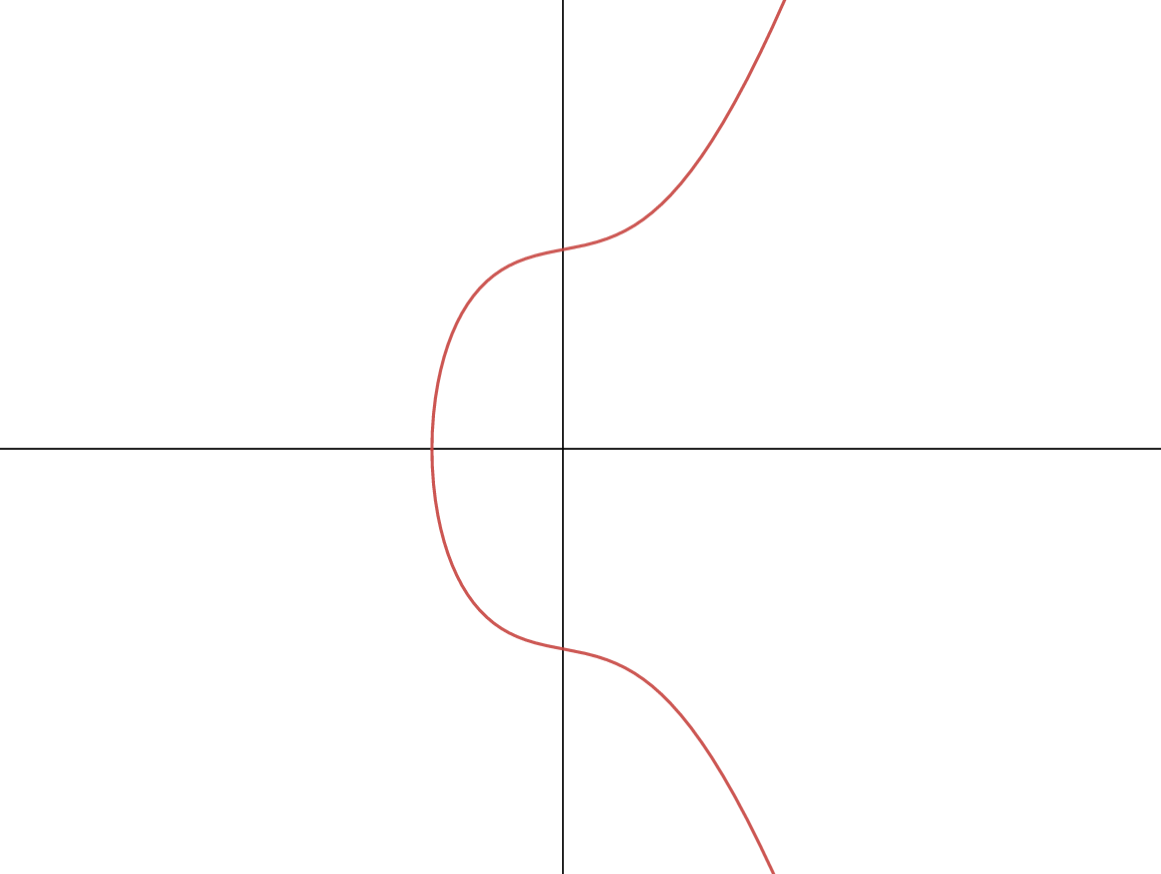
\includegraphics[width=10cm, height=3.3cm]{ECC.png}
 \caption{Elliptic Curve\:\(y^2=x^3+ax+b\)}
\centering
\end{figure}

Elliptic curves cryptography uses elliptic curves over the fintie field \(Z_{p}\)(where \(p\) is prime and \(p>3\)) or \(Z_{2m}\) (where the fields size p=2m).This indicates that the curve's point can only have integer coordinates within the field, which is a square matrix of size \((p*p)\). Each algebric operation performed on the field (such as point addition and multiplication) produces a new point.
% Author --- SABVA JAY DILIPBHAI
\textbf{The Elliptic curve equation over the finite field \(Zp\)}

\hspace{4.5cm}
\begin{centre}
\boxed{\(y^2=x^3+ax+b(mod p)\)}
\end{centre}

\textbf{The Bitcoin curve(secp256k1) equation over the finite field \(Zp\)}

\hspace{4.5cm}
\begin{centre}
\boxed{\(y^2=x^3+7(mod p)\)}
\end{centre}

The ECC uses the points \( (x,y) \) within the Galois field Zp (where x and y are integers in the range [0...p-1]), in comparison to RSA, which uses the integers in the range [0...p-1] for its key space.
% Author --- SABVA JAY DILIPBHAI
\subsection{Mathematics}
Given a curve,E,defined along some equation in a finite field(such as E:\(y^2=x^3+ax+b\),point multiplicatioj is defined as the repeated addition of a point along that curve.denote as \(nP=P+P+P...+P\) for some scalar n and a point \(P=(x,y)\) that lies on  the curve,E.
\subsubsection{Point Operations}

% Author --- SABVA JAY DILIPBHAI
\begin{figure}[hb]
  \centering
  \begin{minipage}[hb]{0.31\textwidth}
    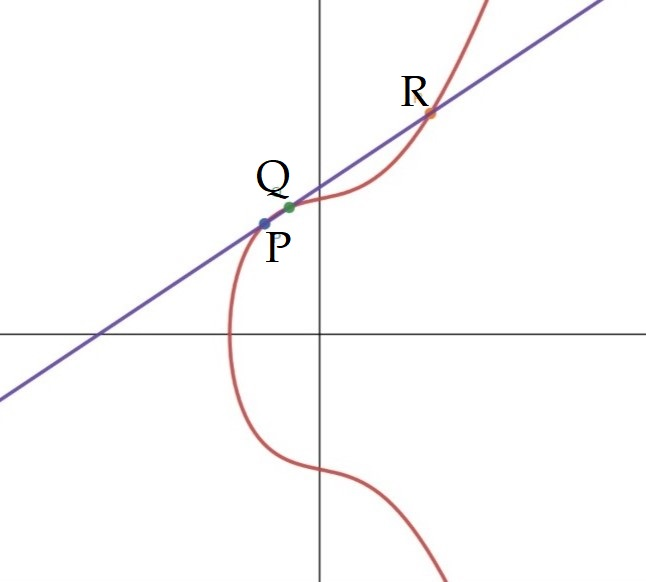
\includegraphics[width=\textwidth]{PQR1.jpeg}
    \caption{       \(P+Q+R=0\)}
  \end{minipage}
  \hfill
  \begin{minipage}[hb]{0.31\textwidth}
    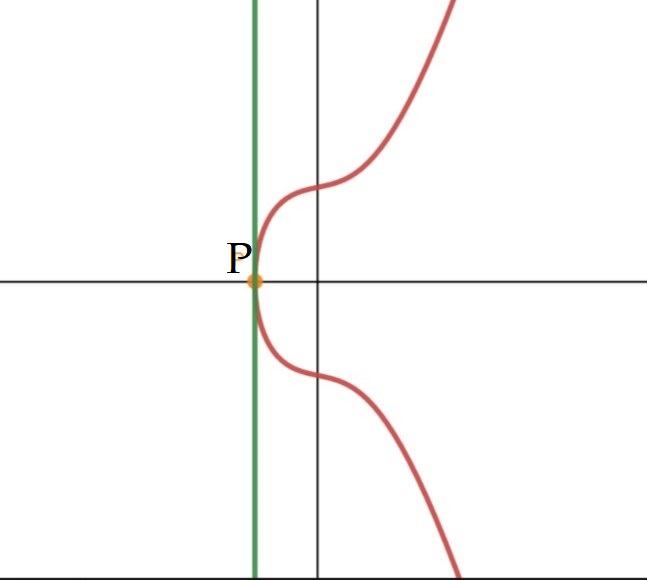
\includegraphics[width=\textwidth]{P.jpeg}
    \caption{  \(P+P+0=0\)}
  \end{minipage}
  
  \begin{minipage}[hb]{0.31\textwidth}
    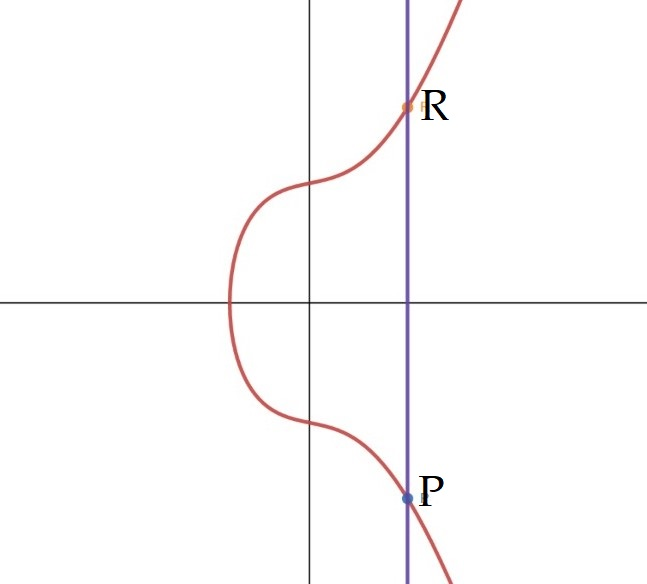
\includegraphics[width=\textwidth]{PR.jpeg}
    \caption{  \(P+R+0=0\)}
  \end{minipage}
  \hfill
  \begin{minipage}[hb]{0.31\textwidth}
    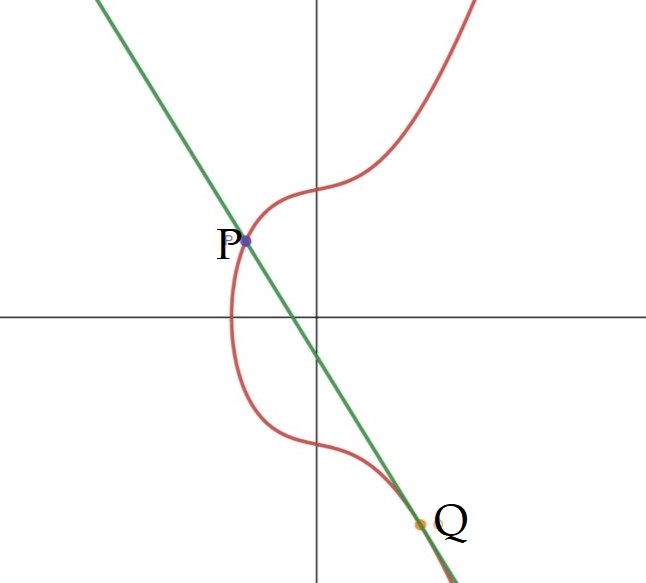
\includegraphics[width=\textwidth]{PQ.jpeg}
    \caption{  \(P+Q+Q=0\)}
  \end{minipage}
  \hfill
  
\end{figure}
\textbf{Point at Infinity}
\newline
Point at infinity \({\mathcal{O}}\) is the identity element of elliptic curve arithmetic.Adding it to ant point result in that other point,including adding point at infinity to itself.That is

\hspace{4cm}
\begin{centre}
\boxed{\({\mathcal{O}}+{\mathcal{O}}={\mathcal{O}}\)}
\newline
\end{centre}

\hspace{4cm}
\begin{centre}
\boxed{\({\mathcal{O}}+{\mathcal{P}}={\mathcal{P}}\)}
\end{centre}

\newline
\textbf{Point negation}
\newline
Point negation is finding such a point,that adding it to itself will result in point at infinity(\({\mathcal{O}}\)).
\begin{figure}[h]
\centering
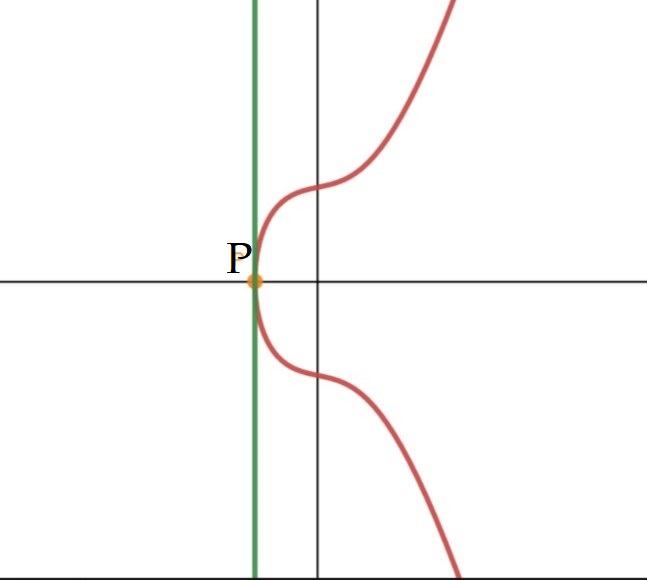
\includegraphics[width=5cm, height=3cm]{P.jpeg}
 \caption{Point negation\:\(P+P+0=0\)}
\centering
\end{figure}

\hspace{4.5cm}
\begin{centre}
\boxed{\({\mathcal{P}}+({\mathcal{-P}})={\mathcal{O}}\)}
\end{centre}

For elliptic curves that is a point with same x coordinate but negated y coordinate:

\begin{centre}
\boxed{\((x,y)+(-(x,y))={\mathcal{O}}\)}
\end{centre}
\begin{centre}
\boxed{\((x,y)+(x,-y))={\mathcal{O}}\)}
\end{centre}
\begin{centre}
\boxed{\((x,-y)=-(x,y)\)}
\end{centre}

\newline
\textbf{Point addition}
\newline
Given Two point in the set
\(E={(x,y)\,|\,y^2+ax+b}\) \cup \:\(\mathcal{O}\)

\begin{figure}[h]
\centering
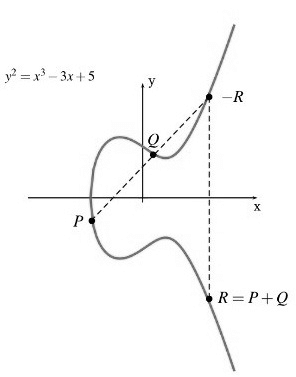
\includegraphics[width=5cm, height=5cm]{Point-Addition-on-the-Elliptic-Curve-18.png}
 \caption{Point addition\:\(P+Q=R\)}
\centering
\end{figure}

With 2 distinct points,$P$ and $Q$,addition is defined as the negation of the point resulting from the intersection of the curve,$E$,and the straight line defined by the points $P$ and $Q$ giving the point,$R$

\hspace{4.3cm}
\begin{centre}
\boxed{$P$\:+ \:$Q$ \:= \:$R$}
\end{centre}

Assuming the elliptic curve,$E$, is given by \(y^2=x^3+ax+b\), so the slope of line ($PQ$) $\lambda$ can be calculated as:
\hspace{3cm}
\begin{center}
    \boxed{\lambda=\frac{y_{q}-y_{p}}{x_q-x_p}}
\end{center}
\hspace{2.5cm}
\begin{centre}
\boxed{x_{r}=\lambda^2-x_{p}-x_{q}}
\end{centre}
\begin{centre}
\boxed{y_{r}=\lambda((x_{p}-x_{r})-y_{p}}
\end{centre}

These equations are correct when neither point is the point at infinity,{\mathcal{O}},and if the points have diffrent x coordinates(they're not mutual inverses).This is important for the Elliptic curve digital singature algorithm(ESDSA) where the hash value could be zero.
\newpage
\textbf{Point doubling}
\newline
Where the point $P$ and $Q$ are coincident(at same coordinate),addition is similar,except that there is no well-defined straight line through $P$,so the operation is closed using limiting case,the tangent to the curve,$E$,at $P$.
\begin{figure}[hb]
  \centering
  \begin{minipage}[hb]{0.3\textwidth}
    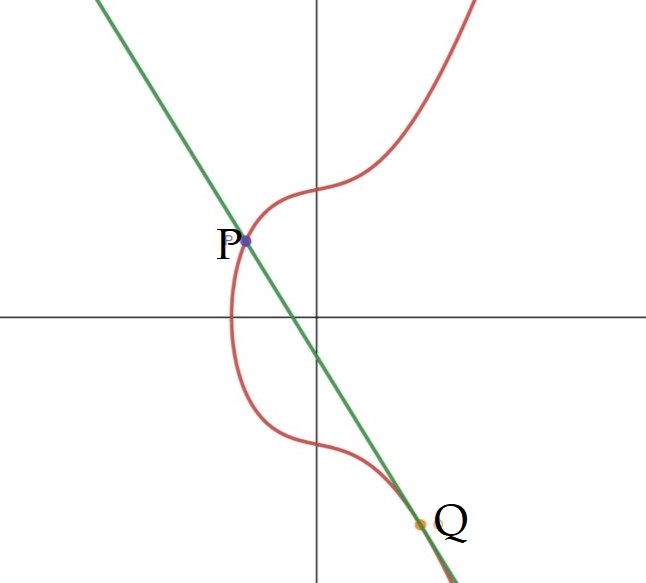
\includegraphics[width=\textwidth]{PQ.jpeg}
    \caption{Point doubling \(P+Q+Q=0\)}
  \end{minipage}
  \hfill
  \begin{minipage}[hb]{0.3\textwidth}
    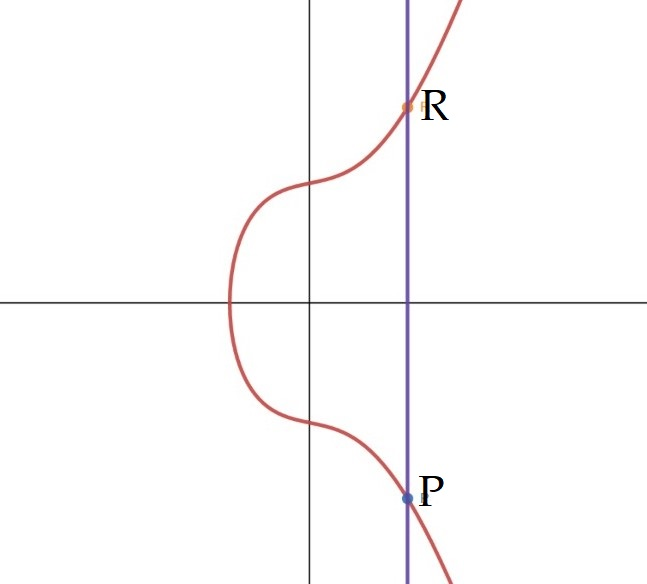
\includegraphics[width=\textwidth]{PR.jpeg}
    \caption{Point doubling \(P+R+0=0\)}
  \end{minipage}
  \hfill
\end{figure}
\begin{comment}
\begin{center}
    \boxed{{\frac{\partial E}{\partial x}}/{\frac{\partial E}{\partial y}}}
\end{center}
\end{comment}
\begin{center}
    \boxed{\lambda=\frac{3x_{p}^2+a}{2y_{p}}}
\end{center}
where a is from the defining equation of the curve,$E$,above.
\newline

\begin{centre}
\hspace{3.1cm}\boxed{x_{r}=\lambda^2-2x_{p}}
\end{centre}
\begin{centre}
\boxed{y_{r}=\lambda((x_{p}-x_{r})-y_{p}}
\end{centre}
\subsubsection{Order and Cofactor of Elliptic Curve}
All the points on an elliptic curve over a finite field can be combined to form a finite cyclic algebraic group. When two EC points from the same cyclic group are combined or multiplied by an integer, the result is another EC point from the same cyclic group (and on the same curve). The order of the curve is determined by the total number of EC points on the curve. The special point known as "$point\:at\:infinity$," which is produced when a point is multiplied by 0, is also included in this total number of points.

Others form a single cyclic group that contains all of the curve's EC points, while other curves generate numerous non-overlapping cyclic subgroups that each contain a portion of the curve's EC points. In the second case, the curve's points are split into h cyclic subgroups, each of order r. (each subgroup holds equal number of points). The overall order of the group is (n=h*r) (the number of subgroup). The number of subgroups h with EC points is denoted by
\textbf{cofactor}.
The cofactor is typically expressed by the following formula:
\begin{center}
    \centering
    \boxed{\(h=n/r\)}
\end{center}

where 
\begin{itemize}
    \item The curve's order is n. (the number of all its points)
    \item The curve cofactor is h. (the number of non-overlapping subgroups of points,which together hold all curve points).
    \item The subgroups are arranged in r. (the number of points in each subgroup,including the infinity point for each subgroup).
\end{itemize}

In other words, the points across an elliptic curve remain in one or more cyclic subgroups, which are non-overlapping subsets. The term "cofactor" refers to the quantity of subgroups. The "order" of the curve, which is often represented by the number n, is the total number of points in all subgroups. If there is just one cyclic subgroup in the curve, then its cofactor h = 1. If the curve has several subgroups, its cofactor is more than 1.
\subsubsection{The Generator Point in ECC}
The ECC cryptosystems define a special pre-defined (constant) EC point called generator point $G$ (base point) for elliptic curves over finite fields. By multiplying $G$ by an integer in the range $[0...r]$, $G$ can create any other point in its subgroup over the elliptic curve. The cyclic subgroup's "order" is represented by the integer $r$. (the total number of all points in the subgroup).

The order $n$ of the curve (the total number of distinct points over the curve, including the infinity), for curves with cofactor=1, is equal to the number $r$. There is only one subgroup for these curves.
% Author --- SABVA JAY DILIPBHAI
When $G$ and $n$ are carefully selected, and the cofactor = 1, all possible EC points on the curve (including the special point infinity) can be generated from the generator $G$ by multiplying it by integer in the range $[1...n]$. This integer n is known as "order of the curve".

It is important to understand that the order r of the subgroup, which might differ from the order of the curve, is what defines the total number of possible private keys for this curve: $r = n / h$. (curve order, divided by the curve cofactor). To ensure that the key space is sufficiently large for a given cryptographic strength, cryptographers carefully choose the elliptic curve domain parameters (curve equation, generating point, cofactor, etc.).

In summary, the EC points and the generator point G together generate cyclic groups (or cyclic subgroups) in the ECC cryptography. This implies that a number $r$ exists (r $>$ 1) such that $r * G = 0 * G = $infinite and all points in the subgroup can be generated by multiplying $G$ by integer in the range [1...r]. Order of the group refers to the number $r$. (or subgroup).
Elliptic curve subgroups typically have a large number of generating points, but cryptographers carefully choose one of them to act as the entire group's (or subgroup's) generator and to allow for performance improvements in the calculations. This is the so-called "$G$" generator.

It is very well known that some curves generate subgroups of varying orders at certain generator points. More specifically, if the group order is $n$, then there exists a point $Q$ such that $d * Q $= infinite for any prime $d$ dividing $n$. As a result, certain locations that are employed as the curve's generators will produce smaller subgroups than others. The security is weak if the group is small. Small-subgroup attacks are what these are called. This is the rationale behind why cryptographers usually select r as a prime integer for the subgroup order.

Different base points can generate numerous subgroups of EC points on elliptic curves with cofactors h $>$ 1 on the curve. The majority of EC point operations and ECC cryptographic methods will function well if we select a certain generator point and operate on that subgroup of points on the curve. It is still advised to use only tried-and-true ECC implementations, algorithms, and software programmes in specific circumstances.
% Author --- SABVA JAY DILIPBHAI

$Generator \:Point \:Example$:

For The EC over finite field \(y^2=x^3+7mod17\),if we take the point G={15,13} as generator,any other point from the curve can be obtained by multiplying G by some integer in the range[1...18].Thus the order of this EC is n=18 and its cofactor h=1.

Note that the curve has 17 normal EC points(shown at the above figure)+one special"point at infinity",all staying in a single subgroup,and the curve order is 18(not 17)

Note also,that if we take the point{5,9} as generator,it will generate just 3 EC points;{5,8},{5,9} and infinity.Because the curve order is not prime number,different generators may generate subgroups of different order.This is a good example why we should not "invent" our own elliptic curves for cryptographic purposes and we should use proven curves.
% Author --- SABVA JAY DILIPBHAI
\subsubsection{Key Generation}
In the ECC, an EC point P is generated by multiplying a fixed EC point G (the generator point) by a certain number k, which may be considered of as a private key (its corresponding public key).

Consequently,in ECC we have:
\begin{itemize}
    \item Elliptic curve (EC) over finite field $Z_{p}$
    \item Generator point= $G$ (fixed constant,a base point on the EC)
    \item Private Key = $k$
    \item Public Key = $P$
\end{itemize}
% Author --- SABVA JAY DILIPBHAI
Using the well-known ECC multiplication methods in time $\mathcal{O}(log2(k))$, such as the "double and add algorithm," $P=k*G$ can be calculated relatively quickly. It will just require a few hundred straight forward EC operations for 256-bit curves.

Calculating $k=P/G$ is extremely time-consuming and is considered to be impossible for big $k$.

The security strength of the ECC cryptography, also known as the ECDLP, is based on this asymmetry (quick multiplication and impractically slow opposite operation) (Discrete Logarithmatic problem).
\section{Commercialization}
Permutations are frequently used in communication networks and parallel and distributed systems . Routing different permutations on a network for performance evaluation is a common problem in these fields. Many communication networks require secure transfer of information, which drives development in cryptography and network security. This area has recently become particularly significant because of the increased use of internet information transfers. Associated problems include protecting the privacy of transactions and other confidential data transfers and preserving the network security from attacks by viruses and hackers. Encryption process involves manipulations of sequences of codes such as digits, characters, and words. Hence, they are closely related to combinatorics, possibly with intelligent encryption process. For example, one common type of encryption process is interchanging--i.e., permuting parts of a sequence . Permutations of fast Fourier transforms are employed in speech encryption . 

Queries in databases are multiple join operations that are permutations of the constituent join operations. Determining an optimal permutation that gives minimum cost is a common and important problem. Data mining or knowledge discovery in databases is a relatively new field that aims at distilling useful information, often from large databases. In this area, techniques employing symbolic AI can manipulate combinatorial sequences of atoms or information elements. Non-symbolic knowledge discovery techniques, such as genetic algorithms and genetic programming, most commonly deal with solutions in the form of sequences of bits, digits, characters, and sometimes Lisp program elements. Neural networks, another domain of non-symbolic AI, sometimes deal with combinatorial patterns. Knowledge discovery techniques under uncertainty, such as Bayesian networks, Dempster-Shafer theory, fuzzy logic, and rough set theory, may have combinatorial solutions.

Some other applications like Computer architecture, Computational molecular biology, Languages, Pattern analysis, Scientific discovery, Operations research, Simulation, Homeland security .


\newline
\newline
\newline
\newline

\section{Evolution of Cryptography}
\begin{center}
    \begin{tabular}{ | l |  p{10cm} |}
    \hline
    Year & Event \\ \hline
    1900 BC & Around 4000 years ago, the Eqyptians used to communicate by messages written in \textbf{hieroglyph}.\\ \hline
    300 BC & "Arthshashtra",a classic work on statecraft written by Kautalya,describes the espionage service in India and mentions giving assignment to spies in "secret writing"\\ \hline
    Wednesday & Rain will still linger for the morning. 
    Conditions will improve by early afternoon and continue 
    throughout the evening. \\
    \hline
    \end{tabular}
\end{center}

\begin{tabularx}{0.9\textwidth} { 
  | >{\raggedright\arraybackslash}X 
  | >{\centering\arraybackslash}X 
  | >{\raggedleft\arraybackslash}X | }
 \hline
 Symmetric Key Size(bits) & RSA-Diffie-Hellman Key Size(bits) & Elliptic Curve Key Size(bits) \\
 \hline
 80 & 1024 & 160 \\
 \hline
 112 & 2048 & 224 \\
 \hline
 128  & 3072  & 256  \\
 \hline
 192 & 7680 & 384 \\
 \hline
 256 & 15360 & 521 \\
 \hline
\end{tabularx}
 

\end{document}
